\documentclass[a4paper,12pt]{extarticle}
\usepackage[table,xcdraw]{xcolor}
\usepackage{pgfplots}
\usepackage[unicode, pdftex]{hyperref}
\usepackage[T2A]{fontenc}
\usepackage[utf8]{inputenc}
\usepackage[english,russian]{babel}
\usepackage{amsmath,amsfonts,amsthm, mathtools}
\usepackage{amssymb}
\usepackage{dsfont}
\usepackage{graphicx}
\graphicspath{{images/}}
\usepackage{wrapfig}
\usepackage{floatrow}
\usepackage{setspace}
\usepackage[headings]{fancyhdr}
\usepackage[margin=10pt,font={small,stretch=0,9},labelfont=bf,labelsep=period,
justification=centerlast]{caption}
\usepackage{array,tabularx,tabulary,booktabs}
\RequirePackage{multirow}
\RequirePackage{multicol}
\RequirePackage{longtable}
\usepackage{indentfirst}
\usepackage{hyperref}
\usepackage{icomma}
\newcommand*{\hm}[1]{#1\nobreak\discretionary{}
	{\hbox{$\mathsurround=0pt #1$}}{}}
\usepackage{soulutf8} 
\usepackage{etoolbox} 
\usepackage{geometry}
\geometry{top=20mm}
\geometry{bottom=20mm}
\geometry{left=20mm}
\geometry{right=20mm}
\DeclareMathOperator{\sgn}{\mathop{sgn}}
\usepackage[OT1]{fontenc}
\usepackage{amsmath}
\usepackage{amsfonts}
\usepackage{amssymb}
\usepackage{wasysym}
\usepackage{wrapfig}
\usepackage{physics}
\usepackage[normalem]{ulem}
\graphicspath{{pictures/}}
\DeclareGraphicsExtensions{.png,.jpg,.jpeg}
\usepackage{indentfirst}
\usepackage[T2A]{fontenc}
\usepackage{subfigure}
\usepackage{fancyhdr}
\usepackage{caption}

\usepackage{tabularx}
\usepackage{floatrow}
\usepackage{multicol}
\usepackage{lastpage}

\pgfplotsset{
  MyStyle1/.style={
    axis lines = middle,
    enlargelimits = true,
    grid=both,
    grid style={line width=.1pt, draw=gray!10},
    major grid style={line width=.2pt,draw=gray!50},
    minor tick num=5,
    enlargelimits=0.05,
    ticklabel style={font=\tiny,fill=white},
    xlabel style={at={(ticklabel* cs:1)},anchor=north west},
    ylabel style={at={(ticklabel* cs:1)},anchor=south east},
  }
}
\def\Slope{1.5}
\def\Intercept{-20}


% Настройка отчёркиваний и нумерации
\usepackage{fancyhdr}
\pagestyle{fancy}
\fancyhf{}

\fancyhead[L]{\nouppercase{\leftmark\hfill}}
\fancyfoot[RO, RE]{Страница \thepage \ из \pageref{LastPage}}
\renewcommand{\headrulewidth}{0.5pt}
\renewcommand{\footrulewidth}{0.5pt}

\usepackage{titlesec}
\titlelabel{\thetitle.\quad}

\pgfplotsset{compat=1.18}
\begin{document}

\thispagestyle{empty}
\begin{center}
	\textit{Федеральное государственное автономное образовательное\\ учреждение высшего образования }
	
	\vspace{0.5ex}
	
	\textbf{«Московский физико-технический институт\\ (национальный исследовательский университет)»}
\end{center}

\vspace{10ex}
\begin{figure}[!h]
  \begin{center}
    
\includegraphics[width = 0.8\textwidth]{MIPT.png}
  \end{center}
\end{figure}

\begin{center}
	
	\textbf{Лабораторная работа № 4.7.2}
	
	\vspace{1ex}
	
	по курсу общей физики
	
	на тему:
	
	\textbf{\textit{<<Эффект Поккельса>>}}
	
	\vspace{20ex}
	
	\begin{flushright}
		\noindent
		\textit{Работу выполнил:}\\  
		\textit{Легких Никита \\(группа Б05-301)}
	\end{flushright}
	\vfill
	Долгопрудный \\ \today
	\setcounter{page}{1}
\end{center}
\newpage

% Конец шаблона
\newpage

\textbf{Цель работы:} исследовать интерференцию рассеянного света, прошедшего кристалл; наблюдать изменение характера поляризации света при наложении на кристалл электрического поля. \\ \\
\textbf{В работе используются:} гели-неоновый лазер, поляризатор, кристалл ниобата лития, матовая пластинка, экран, источник высоко-вольтного переменного и постоянного напряжения (похож на самодельный, серийный номер не найден, руководства тоже, за погрешность берем 1.5-2 цены деления так как, присутствовало трение в стрелке прибора, при постукивании всегда было разное значение, то есть берем погрешность 20 вольт), фотодиод, осциллограф (GWINCTEK GOS-620), линейка (деревянная, знак ГОСТ, не обнаружен, погрешность 1 мм).

\section*{Теоретические сведения и установки}
Эффект Поккельса -- изменение показателя преломления света в кристалле под действием электрического поля.

Рассмотрим кристалл ниобата лития $\text{LiNbO}_3$ с цетральноосевой симметрией вдоль оси $Z$. Для световой волны с $\mathbf{E}$ перпендикулярно $Z$ показатель преломления будет $n_o$, а для волны с $\mathbf{E}$ вдоль $Z$ -- $n_e$. В случае, когда луч света идёт под углом $\theta$ к оси, есть два значение показателя преломления $n_1$ и $n_2$: $n_1 = n_o$ для волны с $\mathbf{E}$ перпендикулярным плоскости $(\mathbf{k},\mathbf{Z})$ (обыкновенная волна) и $n_2$ для волны с $\mathbf{E}$ в этой плоскости (необыкновенная волна). В последнем случае
\begin{equation}
\dfrac{1}{n_2^2}=\dfrac{\cos^2 \theta}{n_0^2}+\dfrac{\sin^2 \theta}{n_e^2}.
\end{equation}

\begin{figure}[h]
	\center{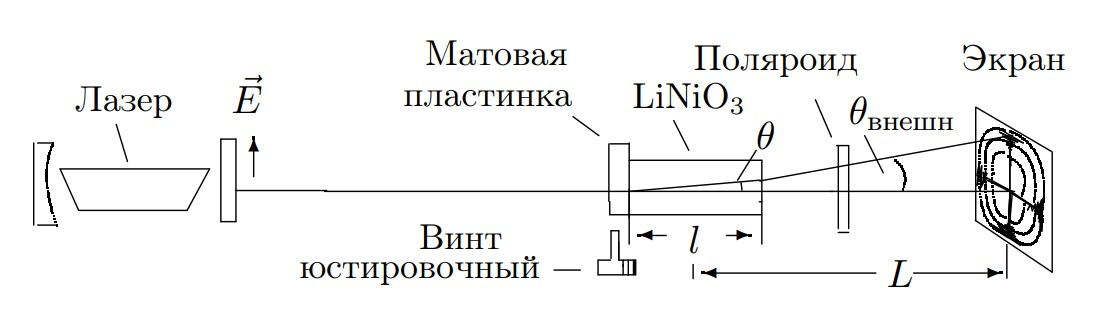
\includegraphics[scale=0.5]{pics/1.jpg}}
  \caption{\centering Оптическая часть экспериментальной установки}
	\label{fig:image1}
\end{figure}

Если перед кристаллом, помещённым между поляроидами, расположить линзу или матовую пластинку, то на экране за поляроидом мы увидим тёмные концентрические окружности -- результат интерференции обыкновенной и необыкновенной волн. При повороте выходного поляроида на $90^\circ$ картина меняется с позитива на негатив (на месте светлых пятен появляются тёмные и наоборот). В случае, когда разрешённое направление анализатора перпендикулярно поляризации лазерного излучения, радиус тёмного кольца с номером $m$ равен
\begin{equation}
r_m^2 = \dfrac{\lambda}{l} \dfrac{(n_oL)^2}{n_0 - n_e}m,
\end{equation}

\begin{figure}[h]
	\center{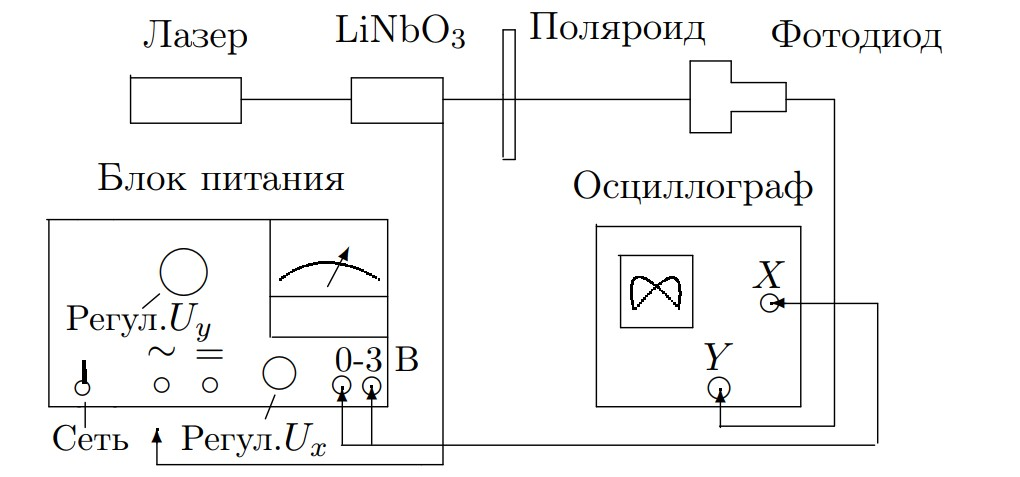
\includegraphics[scale=0.5]{pics/2.jpg}}
 \caption{\centering Экспериментальная установка}
	\label{fig:image1}
\end{figure}

где $L$ -- расстояние от центра кристалла до экрана, $l$ -- длина кристалла.

Теперь поместим кристалл в постоянное электрическое поле $E_{\text{эл}}$, направленное вдоль оси $X$, перпендикулярной $Z$. Показатель преломления для луча, распространяющего вдоль $Z$, всегда $n_o$. В плоскости $(X,Y)$ возникают два главных направления под углами $45^\circ$ к $X$ и $Y$ с показателями преломления $n_0 - \Delta n$ и $n_o + \Delta n$ (быстрая и медленная ось), причём $\Delta n = A E_{\text{эл}}$. Для поляризованного вертикально света и анализатора, пропускающего горизонтальную поляризацию, на выходе интенсивность на выходе будет иметь вид
\begin{equation}
I_{\text{вых}} = I_0 \sin^2 \left(\dfrac{\pi}{2} \dfrac{U}{U_{\lambda/2}} \right),
\end{equation}
где $\displaystyle U_{\lambda/2} = \frac{\lambda}{4A}\frac{d}{l}$ -- \textit{полуволновое напряжение}, $d$ -- поперечный размер кристалла.  При напряжении $U = E_{\text{эл}}d$ равном полуволновому сдвиг фаз между двумя волнами равен $\pi$, а интенсивность света на выходе максимальна. 


На Рис. 2 представлена схема всей установки (оптическая часть изорбажена на Рис. 1). Свет лазера, проходя через сквозь пластину, рассеивается и падает на двоякопреломляющий кристалл. На экране за поляроидом видна интерференционная картина. Убрав рассеивающую пластину и подавая на кристалл постоянное напряжение, можно величиной напряжения влиять на поляризацию луча, вышедшего из кристалла. Заменив экран фотодиодом и подав на кристалл переменное напряжение, можно исследовать поляризацию с помощью осциллографа.

\section*{Задание}
\subsection*{Измерение радиусов темных колец}
Соберем установку по схеме, изображенной на рис.1, проведем юстировку системы. Далее получим интерференционную картину для расстояния $L =  71.5 \pm 1.0$ см (от середины кристалла до экрана). Проведем измерения внешних и внутренних диаметров тёмных колец, результаты внесем в таблицу ниже: 
\begin{table}[H]
\begin{tabular}{|c|c|c|}
\hline
m & $d_{\text{внут}}$, см & $d_{\text{внеш}}$, см \\ \hline
1 & 5.0    & 5.8    \\ \hline
2 & 7.4    & 7.8    \\ \hline
3 & 9.0    & 9.5    \\ \hline
4 & 10.5   & 10.9   \\ \hline
5 & 11.8   & 12.2   \\ \hline
\end{tabular}
\end{table}
Теперь наша задача построить график $r_2 = f(m)$. По углу наклона прямой определим
двулучепреломление $(n_o - n_e)$ ниобата лития, пользуясь формулой (2), делаем по следующим данным:
$\lambda = 0,63$ мкм, $l = 26$ мм, $n_o = 2.29$
\begin{table}[H]
\begin{tabular}{|c|c|c|c|c|c|}
\hline
$m$  & 1  & 2  & 3  & 4   & 5   \\ \hline
$r^2$, см$^2$       & 29 & 58 & 86 & 114 & 144 \\ \hline
$\Delta r^2$, см$^2$ & 4  & 3  & 5  & 4   & 5   \\ \hline
\end{tabular}
\end{table}
\begin{minipage}{1\textwidth}
      \begin{tikzpicture}
        \begin{axis}[
          width=0.6\textwidth,
          height=,
          xlabel={$m$},
          ylabel={$r^2$, см$^2$},
          MyStyle1,
          ]
          \draw[blue, domain=0:100] plot (\x,7.3*\x-0.5);
          \addplot[purple, only marks] plot [error bars/.cd,
                x dir=both, x fixed = 0,
                y dir=both, y explicit,
                      ] table [
                      x=m, y=r2,
                x error minus=null, x error plus=null, y error minus=err_r2, y error plus=err_r2, col sep=comma] {data/m-r2.csv};
        \end{axis}
      \end{tikzpicture}
    \end{minipage}
Угол наклона и погрешность оцениваем методом взвешенного МНК, получаем:
$$ \alpha = (7.3\pm0.1) \text{см}^2 = \frac{\lambda}{l} \cdot \frac{(n_o L)^2}{n_o - n_e}$$
откуда получаем что $(n_e - n_o) = (0,096 \pm 0,008)$, погрешность берем по формуле: \\ $\Delta (n_e - n_o) = (n_e - n_o) \cdot \frac{\Delta \alpha}{\alpha} \cdot 2\frac{\Delta L}{L}$

В то время как табличное значение равно $0.09$, а значит, они равны в пределах погрешностей.

\subsection*{Определение полуволнового напряжения}
Теперь перейдём ко второй части эксперимента.
Подключим разъём блока питания на постоянное напряжение, установим
регулятор напряжения на минимальное напряжение и включим блок питания в сеть.
Для перпендикулярных и параллельных поляризаций лазера и анализатора проделаем опыт с увеличением напряжения на кристалле и измерением максимумов и минимумов интенсивности.

Полученные результаты
внесем в таблицу ниже:
\begin{table}[H]
\centering
\begin{tabular}{|l|l|l|}
\hline
  & $U_{\text{парал}}$, В & $U_{\text{перп}}$, В \\ \hline
$U_{\lambda/2}$  & 405                     & 430                  \\ \hline
$U_{\lambda}$    & 855                     & 870                  \\ \hline
$U_{3\lambda/2}$ & 1330                  & 1350                \\ \hline
\end{tabular}
\end{table}
Разница между параллельной и перпендикулярной поляризациями укладывается в погрешность, поэтому говорить о физическом смысле нет мотивации.

Вместо экрана ставим фотодиод и подключаем его в Y выход осциллографа, получаем вид фигур Лиссажу, определяющийся формулой (3). С помощью этого метода определяем значения $U_{\lambda}, U_{\lambda/2}, U_{3\lambda/2}$ и занесем их в общую таблицу: 
\begin{table}[H]
\centering
\begin{tabular}{|l|l|l|l|}
\hline
  & $U_{\text{парал}}$, В & $U_{\text{перп}}$, В & $U_{\text{Лиссажу}}$, В\\ \hline
$U_{\lambda/2}$  & 405                     & 430        & 390          \\ \hline
$U_{\lambda}$    & 855                     & 870        & 850          \\ \hline
$U_{3\lambda/2}$ & 1330                  & 1350         & 1320       \\ \hline
\end{tabular}
\end{table}

Видно что значения очень близки друг к другу, значит принцип определения напряжений полуволн из фигур Лиссажу верен. 
\begin{figure}[H]
    \centering
    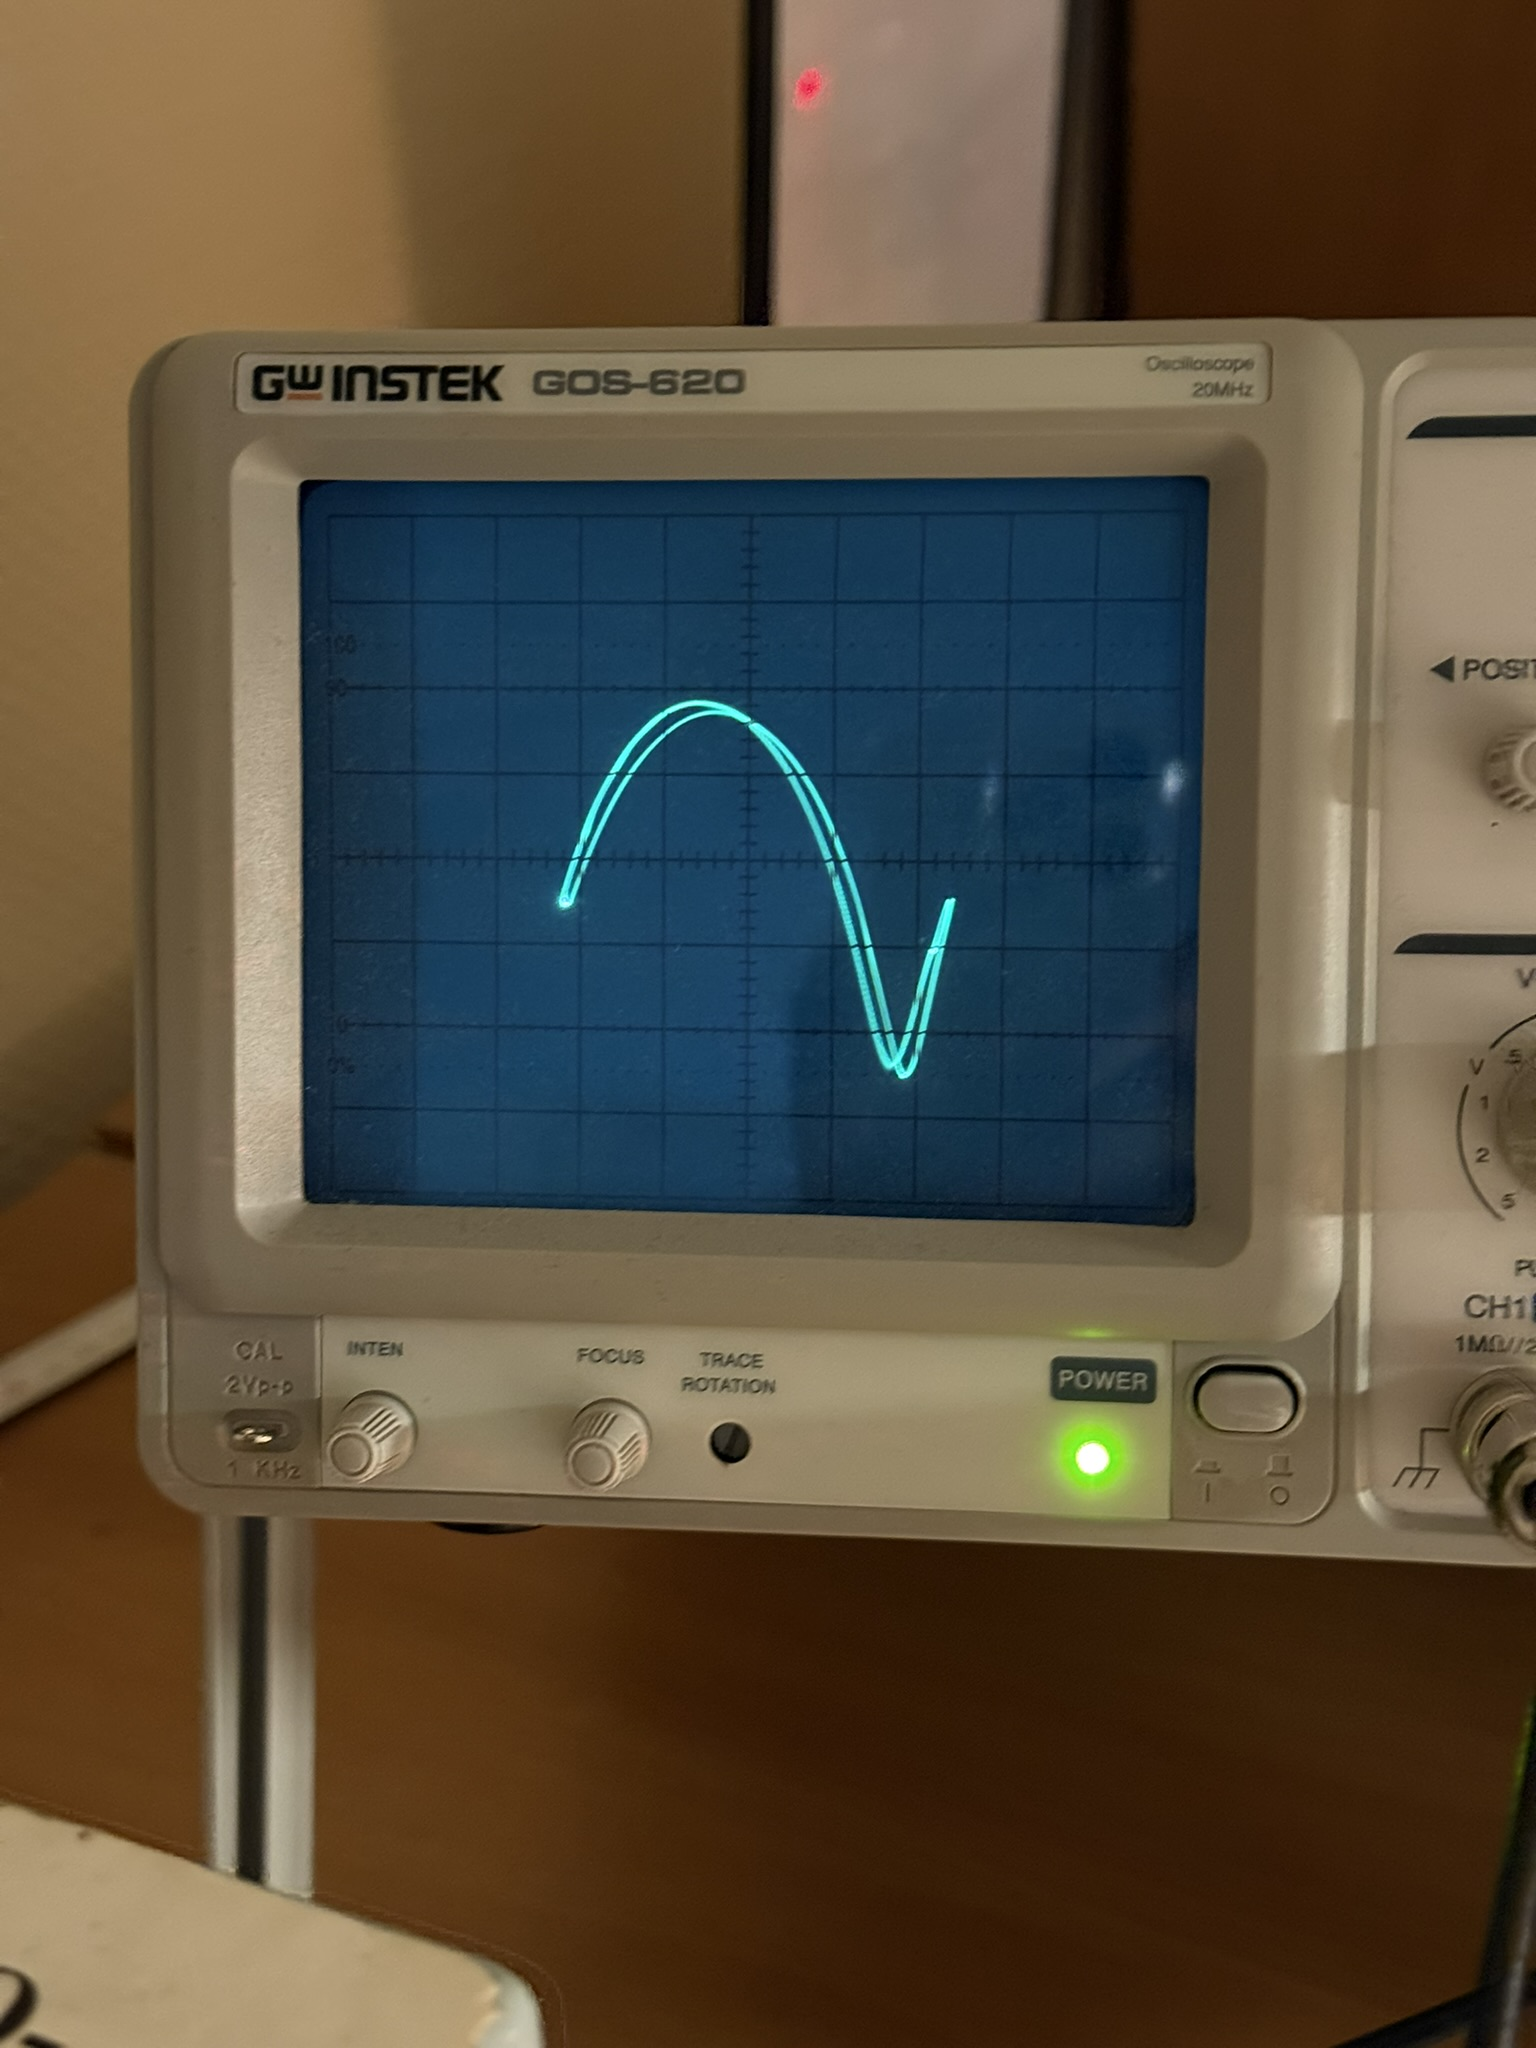
\includegraphics[width=0.3\linewidth]{pics/lis1-2.jpeg}
    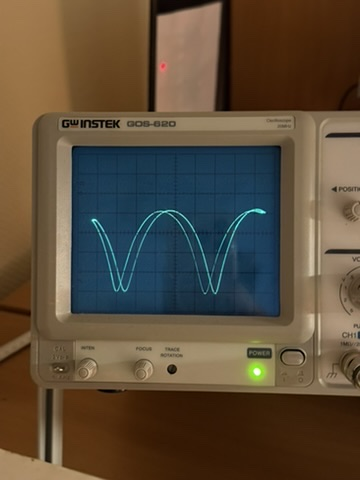
\includegraphics[width=0.3\linewidth]{pics/lis1-1.jpeg}
    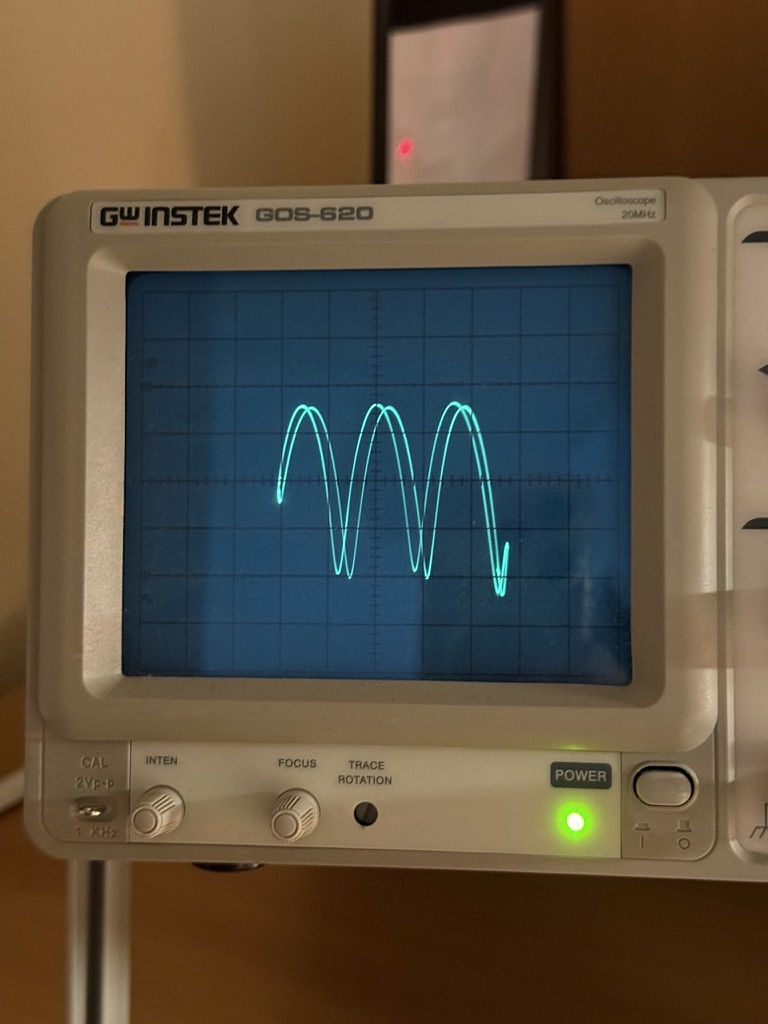
\includegraphics[width=0.3\linewidth]{pics/lis3-2.jpeg}
    \caption{слева направо: $\lambda/2, \lambda, 3\lambda/2$}
\end{figure}

\section*{Вывод}
В ходе данной работы была исследована интерференция рассеянного света, прошедшего сигнал. Также при помощи исследования зависимости
радиуса тёмного кольца от его номера, было вычислено двулучепреломление кристалла, равное $n_o - n_e = (0, 096 \pm 0, 012)$ В, что находится достаточно близко к табличному значению(0, 09 В).


Также была получена сводная таблица напряжений: 
\begin{table}[H]
\centering
\begin{tabular}{|l|l|l|l|}
\hline
  & $U_{\text{парал}}$, В & $U_{\text{перп}}$, В & $U_{\text{Лиссажу}}$, В\\ \hline
$U_{\lambda/2}$  & 405                     & 430        & 390          \\ \hline
$U_{\lambda}$    & 855                     & 870        & 850          \\ \hline
$U_{3\lambda/2}$ & 1330                  & 1350         & 1320       \\ \hline
\end{tabular}
\end{table}, где как видно все соответствующие значения лежат близко к друг другу, в пределах погрешности нащего генератора. 

Также было подтверждено, что при изменении поляризации с паралельной на перпендикулярную не фигура Лиссажу переходит из косинусоиды в синусоиду и наоборот.
\end{document}